\documentclass[12pt,a4paper]{article}

% include standard packages:
\usepackage{graphicx, epstopdf} % eps... for e.g. MATLAB-Grafiken im .eps-format
\graphicspath{{./img/}} % default folder for images

\usepackage{xcolor}
\usepackage{hyperref} % [colorlinks,linkcolor=black,citecolor=black,urlcolor=black] % customize references
\usepackage{amsmath, amsfonts, amssymb, amsthm} % enhanced math writing
\usepackage{tikz-timing} % Timing, Square-Symbols
\usepackage[clock, weather, misc, alpine, geometry, electronic]{ifsym} % \showclock; \Sun; \Letter; \Hut; \FallingEdge
\usepackage{wasysym,gensymb,trfsigns} % Celsius, Hantelsymb.
\usepackage[tmargin=1in,bmargin=1in,lmargin=1.25in,rmargin=1.25in]{geometry} % MSWord-Format
\setlength{\parindent}{0em} % keine Einrueckungen, sonst \noindent
\usepackage{titling} % customize title
\renewcommand\maketitlehooka{\null\mbox{}\vfill}
\renewcommand\maketitlehookd{\vfill\null}

\usepackage{listings, lstautogobble} % adding code listing support
\newcommand*\listingspath[1]{\lstset{inputpath=#1}}
\listingspath{./codes/} % default folder for codes

\usepackage{float} % improved inteferce of floating objects (e.g. \floatplacement{figure}{H})
\usepackage{sectsty} % apply different fonts for a section
\usepackage{eso-pic} % backround image e.g.
\usepackage{ulem} % \uuline = Doppelt unterstreichen
\usepackage{tikz} % drawing things
\usepackage{pgfplots} % plots, graphs, etc.
\usepackage{pdfpages} % include image as pdf

% customize Header and Footer
\usepackage{fancyhdr, lastpage}
\pagestyle{fancy}
\fancyhf{}
\lhead{MCSD - Project Documentation}
\rhead{Jonas Berger}
\lfoot{\today}
\rfoot{Seite \thepage \space von \pageref{LastPage}}
\renewcommand{\headrulewidth}{0.4pt}
\renewcommand{\footrulewidth}{0.4pt}

% Umlaute-Encoding und Standardschrift einstellen:
\usepackage[ngerman]{babel}
\usepackage[utf8]{inputenc}
\usepackage[T1]{fontenc}
\usepackage{lmodern}

% uncomment the following 2 lines to use Arial
%\usepackage{helvet}
%\renewcommand{\familydefault}{\sfdefault}

% Rename listings
%\renewcommand{\contentsname}{Inhaltsverzeichnis}
\renewcommand{\lstlistlistingname}{Codelisting}
%\renewcommand{\listfigurename}{Abbildungsverzeichnis}

% Add listoffigures and codelistings in tableofcontents
\usepackage[nottoc,numbib]{tocbibind}
\renewcommand{\lstlistoflistings}{\begingroup
	\tocfile{\lstlistlistingname}{lol}
\endgroup}

% Code insertion
\usepackage{matlab-prettifier} % for MATLAB
\definecolor{mygreen}{rgb}{0,0.6,0}
\definecolor{mygray}{rgb}{0.5,0.5,0.5}
\definecolor{mymauve}{rgb}{0.58,0,0.82}

\lstdefinestyle{customC}{
	backgroundcolor=\color{white},   % choose the background color; you must add \usepackage{color} or \usepackage{xcolor}; should come as last argument
	basicstyle=\scriptsize,        % the size of the fonts that are used for the code
	breakatwhitespace=false,         % sets if automatic breaks should only happen at whitespace
	breaklines=true,                 % sets automatic line breaking
	captionpos=b,                    % sets the caption-position to bottom
	columns=fullflexible,
	commentstyle=\color{mygreen},    % comment style
	deletekeywords={...},            % if you want to delete keywords from the given language
	escapeinside={\%*}{*)},          % if you want to add LaTeX within your code
	extendedchars=true,              % lets you use non-ASCII characters; for 8-bits encodings only, does not work with UTF-8
	firstnumber=1,                % start line enumeration with line 1
	frame=single,	                   % adds a frame around the code
	identifierstyle=\ttfamily,
	inputencoding=utf8,
	keepspaces=true,                 % keeps spaces in text, useful for keeping indentation of code (possibly needs columns=flexible)
	keywordstyle=\color{blue},       % keyword style
	language=C,                 % the language of the code
	literate=
	{á}{{\'a}}1 {é}{{\'e}}1 {í}{{\'i}}1 {ó}{{\'o}}1 {ú}{{\'u}}1
	{Á}{{\'A}}1 {É}{{\'E}}1 {Í}{{\'I}}1 {Ó}{{\'O}}1 {Ú}{{\'U}}1
	{à}{{\`a}}1 {è}{{\`e}}1 {ì}{{\`i}}1 {ò}{{\`o}}1 {ù}{{\`u}}1
	{À}{{\`A}}1 {È}{{\'E}}1 {Ì}{{\`I}}1 {Ò}{{\`O}}1 {Ù}{{\`U}}1
	{ä}{{\"a}}1 {ë}{{\"e}}1 {ï}{{\"i}}1 {ö}{{\"o}}1 {ü}{{\"u}}1
	{Ä}{{\"A}}1 {Ë}{{\"E}}1 {Ï}{{\"I}}1 {Ö}{{\"O}}1 {Ü}{{\"U}}1
	{â}{{\^a}}1 {ê}{{\^e}}1 {î}{{\^i}}1 {ô}{{\^o}}1 {û}{{\^u}}1
	{Â}{{\^A}}1 {Ê}{{\^E}}1 {Î}{{\^I}}1 {Ô}{{\^O}}1 {Û}{{\^U}}1
	{ã}{{\~a}}1 {ẽ}{{\~e}}1 {ĩ}{{\~i}}1 {õ}{{\~o}}1 {ũ}{{\~u}}1
	{Ã}{{\~A}}1 {Ẽ}{{\~E}}1 {Ĩ}{{\~I}}1 {Õ}{{\~O}}1 {Ũ}{{\~U}}1
	{œ}{{\oe}}1 {Œ}{{\OE}}1 {æ}{{\ae}}1 {Æ}{{\AE}}1 {ß}{{\ss}}1
	{ű}{{\H{u}}}1 {Ű}{{\H{U}}}1 {ő}{{\H{o}}}1 {Ő}{{\H{O}}}1
	{ç}{{\c c}}1 {Ç}{{\c C}}1 {ø}{{\o}}1 {å}{{\r a}}1 {Å}{{\r A}}1
	{€}{{\euro}}1 {£}{{\pounds}}1 {«}{{\guillemotleft}}1
	{»}{{\guillemotright}}1 {ñ}{{\~n}}1 {Ñ}{{\~N}}1 {¿}{{?`}}1 {¡}{{!`}}1,
	morekeywords={*,...},            % if you want to add more keywords to the set
	numbers=none,                    % where to put the line-numbers; possible values are (none, left, right)
	numbersep=5pt,                   % how far the line-numbers are from the code
	numberstyle=\tiny\color{mygray}, % the style that is used for the line-numbers
	rulecolor=\color{black},         % if not set, the frame-color may be changed on line-breaks within not-black text (e.g. comments (green here))
	showspaces=false,                % show spaces everywhere adding particular underscores; it overrides 'showstringspaces'
	showstringspaces=false,          % underline spaces within strings only
	showtabs=false,                  % show tabs within strings adding particular underscores
	stepnumber=1,                    % the step between two line-numbers. If it's 1, each line will be numbered
	stringstyle=\color{mymauve},     % string literal style
	tabsize=2,	                   % sets default tabsize to 2 spaces
	title=\lstname,                   % show the filename of files included with \lstinputlisting; also try caption instead of title
	autogobble=true            % autoalign text
}

\lstset{style=customC} % use customC-style as source-code highlighter for code

% set up \maketitle to accept a new item
\predate{\begin{center}\placetitlepicture\large}
	\postdate{\par\end{center}}

% commands for including the picture
\newcommand{\titlepicture}[2][]{%
	\renewcommand\placetitlepicture{%
		\includegraphics[#1]{#2}\par\medskip
	}%
}
\newcommand{\placetitlepicture}{} % initialization



\begin{document}
% Title page configuration
\title{Project Documentation: \\ Temperature-Measuring and Visualization System}
\author{Jonas Berger}
\date{Datum: \today}
\titlepicture[width=0.9\linewidth]{title_img}

\maketitle

\thispagestyle{empty}
\pagebreak

\renewcommand{\abstractname}{Abstract}
\begin{abstract}
	\noindent
	Diese Dokumentation soll das  Projekt "Temperature-Measuring and Visualization System"\space beschreiben.
	Dabei werden theoretische Vorkenntnisse, Schaltpläne, die konkrete Implementierung, etwaige Messungen und ein "Lessons Learned"\space dokumentiert.
\end{abstract}

\tableofcontents
\pagebreak

\section{Projektspezifikation}
 Das nachfolgende Blockschaltbild \ref{figure:blockschaltbild} zeigt vereinfacht alle verwendeten Bauteile, Sensoren und Anzeigen mit entsprechenden Bussystemen bzw. Ansteuerungen:

\begin{figure}[H]
	\centering
	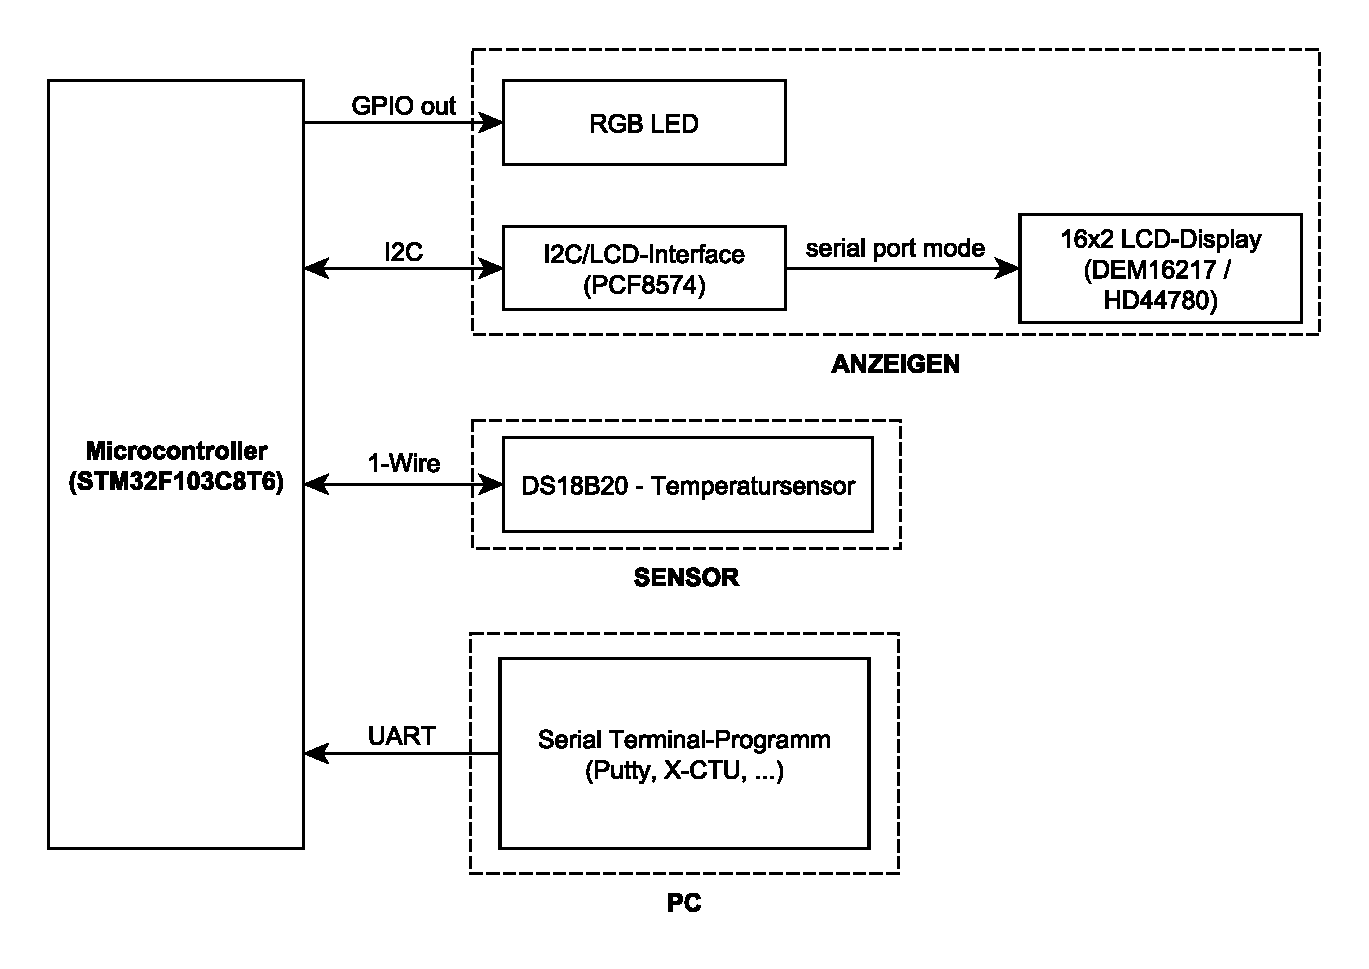
\includegraphics[width=1\linewidth]{Project_Mockup_V05}
	\caption{Blockschaltbild}
	\label{figure:blockschaltbild}
\end{figure}

Zunächst soll die aktuelle Temperatur mit dem DS18B20-Temperatursensor über das 1-Wire-Protokoll ausgelesen werden. Dieser Wert soll auf ein 16x2 LCD-Display ausgegeben werden. \\
Jedoch wird der Wert nicht direkt vom Microcontroller an das Display übertragen, sondern wird an den $\mathrm{I^{2}C}$-to-LCD Interface-Baustein (PCF8574) via $\mathrm{I^{2}C}$ gesendet. Damit wird ein hoher Verbrauch von Portleitungen des Microcontrollers zur Ansteuerung des Displays vermieden. \\
\\ Ein weiteres Feature ist die Einstellung einer Solltemperatur via UART-Protokoll über einen angeschlossenen PC mit einem Serial-Terminal-Programm. Dieser Wert wird ebenfalls am LCD-Display angezeigt. \\
Sollte sich die gemessene Temperatur innerhalb einer gewissen Toleranz befinden leuchtet eine RGB-LED grün. Ansonsten werden größere Abweichungen vom Sollwert stufenweise grün-rot bis rot angezeigt.
\pagebreak

\section{Verwendete Hardware}
Folgende Hardware wird in dem Projekt verwendet:
\begin{itemize}
	\item STM32F103C8T6-Microcontroller
	\item 16x2 LCD-Display (z.B. HD44780, DEM16217, ...)
	\item I2C/LCD-Interface Baustein (verwendet PCF8574-Chip)
	\item RGB-LED (KY-016)
	\item DS18B20 1-Wire-Temperatursensor
	\item PC mit Serial-Terminal-Programm (z.B. Putty, X-CTU, ...)
\end{itemize}

\section{Schematic}
In folgender Abbildung ist die gesamte Schaltung ersichtlich:
\begin{figure}[H]
	\centering
	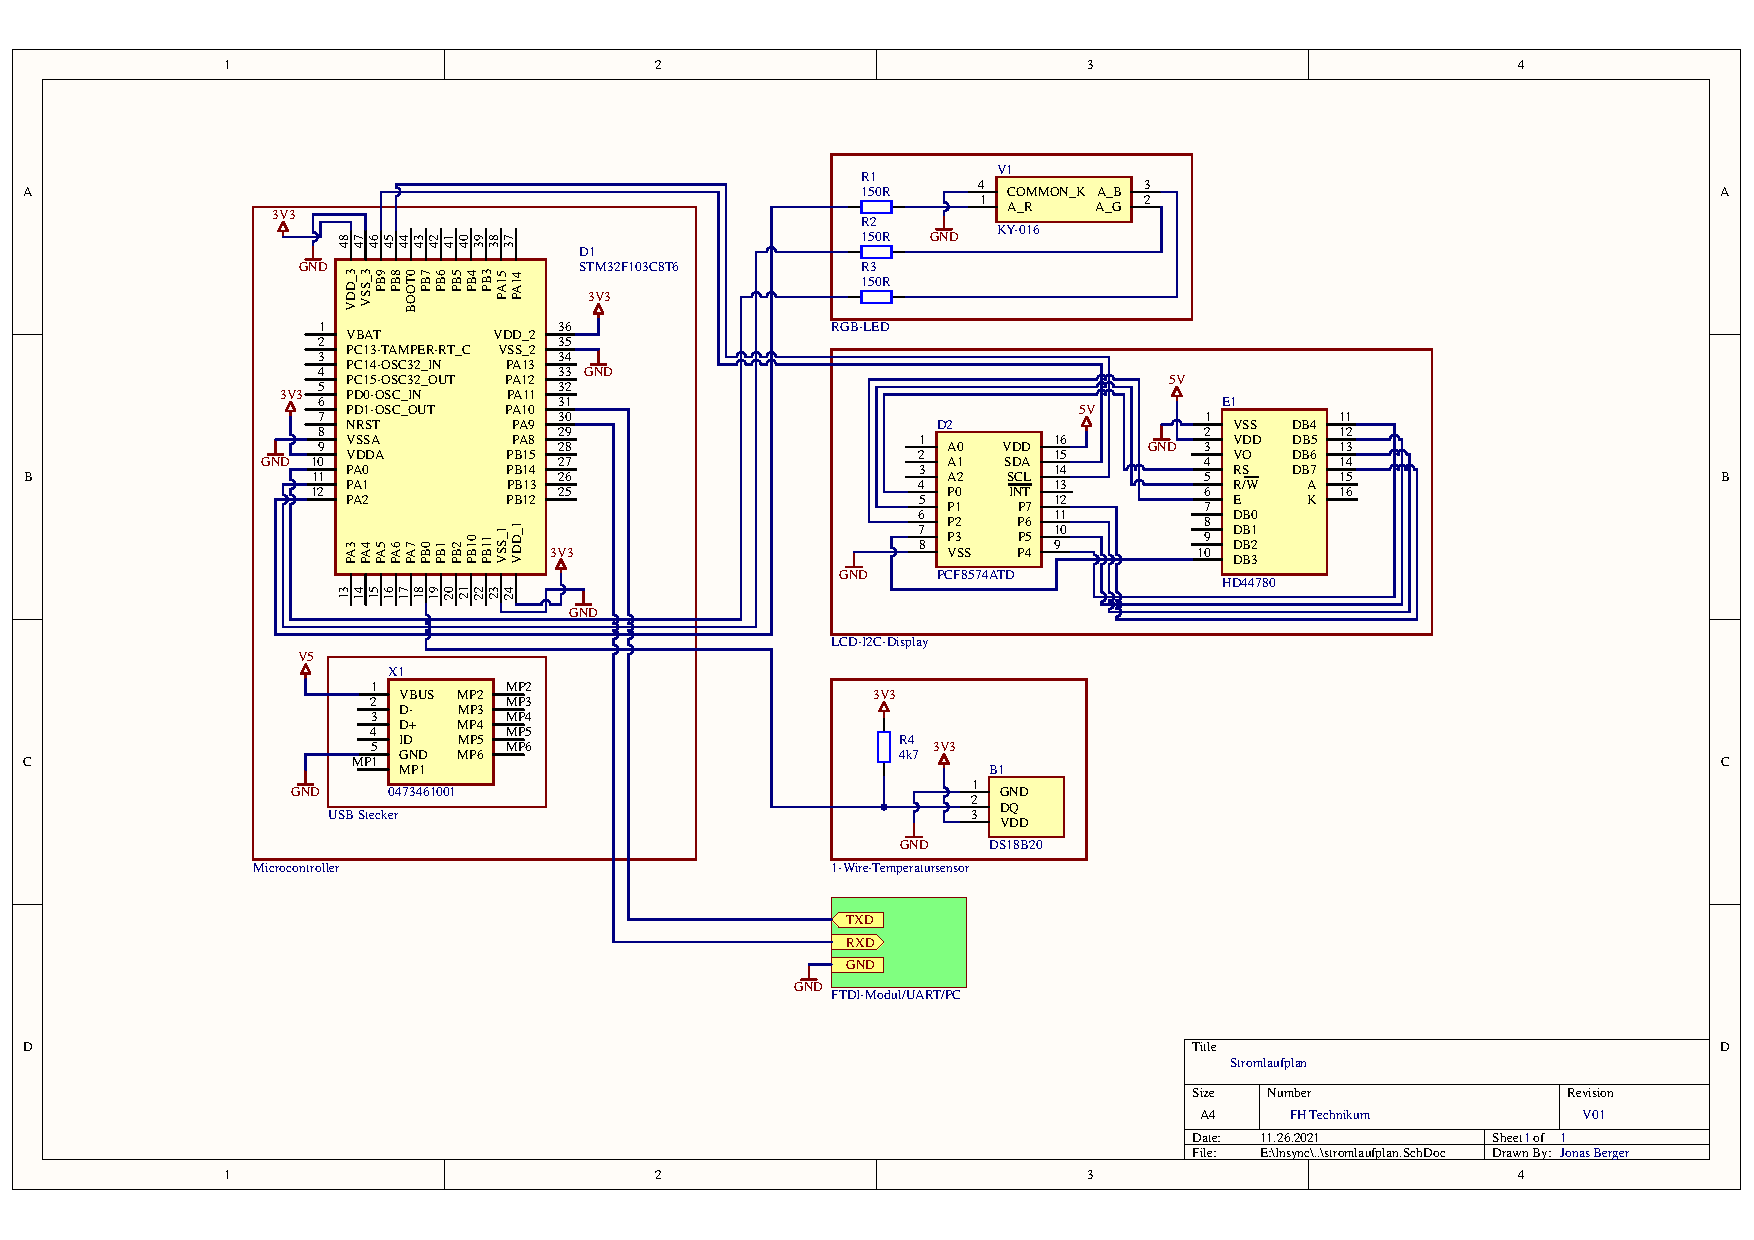
\includegraphics[clip, trim={3cm 4cm 5cm 2cm}, width=1\textwidth]{stromlaufplan_V01.pdf} % trim={<left> <lower> <right> <upper>}
	\caption{Project Schematic}
	\label{figure:schematic}
\end{figure}

\pagebreak

\section{Theorie}
\subsection{Bit banding}
Die Cortex-M3-Memory-Map enthält zwei Bitbandbereiche. Jedes Bit im Bitband-Speicherbereich wird einem Word im Alias-Speicherbereich zugeordnet. Wird das Word im Alias-Bereich beschrieben, so hat das den gleichen Effekt wie eine Read-Modify-Write-Operation auf das Zielbit in der entsprechenden Bitbandregion.\\
\\Folgende Mapping-Formula wird zur Berechnung der Bit-Band-Adresse verwendet:\\
$\text{bit\_word\_addr} = \text{bit\_band\_base} + (\text{byte\_offset} \times 32) + (\text{bit\_number} \times 4)$

\begin{itemize}
	\item bit\_word\_addr is the address of the word in the alias memory region that maps to the targeted bit.
	\item bit\_band\_base is the starting address of the alias region
	\item byte\_offset is the number of the byte in the bit-band region that contains the targeted bit
	\item bit\_number is the bit position (0-7) of the targeted bit.
\end{itemize}

\subsection{1-Wire-Protokoll}
Das 1-Wire-Protokoll ist ein asynchroner, bidirektionaler und half-duplex serieller Datenbus, der nach dem Master-Slave-Prinzip funktioniert und von der Firma DALLAS Semiconducter Corp. entwickelt wurde. Das Protokoll verwendetet dabei nur eine Leitung für die Datenübertragung und zwingend eine Ground-Leitung. Je nach 1-Wire-Slave wird auch eine eigene Versorgungsleitung benötigt, sonst können viele 1-Wire-Bauteile auch direkt die Datenleitung als Versorgung verwenden. Diesen Betrieb nennt man auch "Parasitären Betrieb". \\
Da es keine CLK-Leitung gibt, arbeitet dieser Bus mit eine Zeitschlitzverfahren. Die Übertragung eines Bits dauert standardmäßig 60$\mu$s (6$\mu$s im Overdrive-Modus). Zwischen logisch "0"\space und "1"\space wird unterschieden, je nachdem wie lange die DQ-Leitung auf "Low"\space ist. \\
\\Nachstehend ist der OneMaster-MultipleSlaves-Aufbau ersichtlich:

\begin{figure}[H]
	\centering
	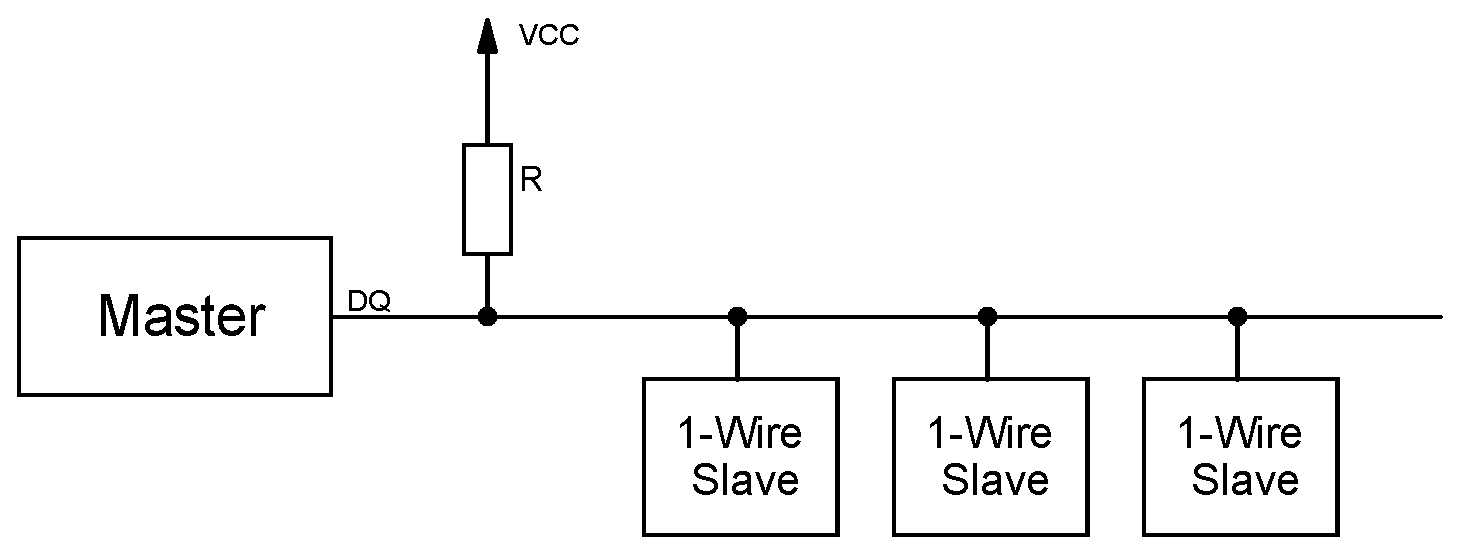
\includegraphics[width=0.9\linewidth]{one_wire.eps}
	\caption{1-Wire Master/Slaves}
	\label{figure:onewire}
\end{figure}

\pagebreak

\subsection{I$^2$C-Schnittstelle}
Die I$^2$C-Schnittstelle ist eine weitverbreite Microcontroller-Peripherie-Schnittstelle, die von Phillips entwickelt wurde. Sie verwendet zwei Leitungen zur Datenübertragung, die jeweils mit einem Pull-Up Widerstand auf die Versorgungsspannung gezogen werden. Dabei erfolgt über die SDA-Leitung der bidirektionale Datenverkehr und über die SCL-Leitung wird der Takt übertragen. \\ Einzelne angeschlossene Peripheriebausteine werden über eine 7-Bit Adresse angesteuert, dass zu einer maximalen Slave-Anzahl von 112 führt, da 16 reserviert sind. Weiters verfügt die Schnittstelle über fünf unterschidliche Geschwindigkeitsmodi, nämlich Standard Mode, Fast Mode, Fast Mode Plus, High Speed Mode und Ultra Fast-mode, womit Datenübertragungsraten von 0,1 Mbit/s bis 5,0 Mbit/s möglich sind.

\begin{figure}[H]
	\centering
	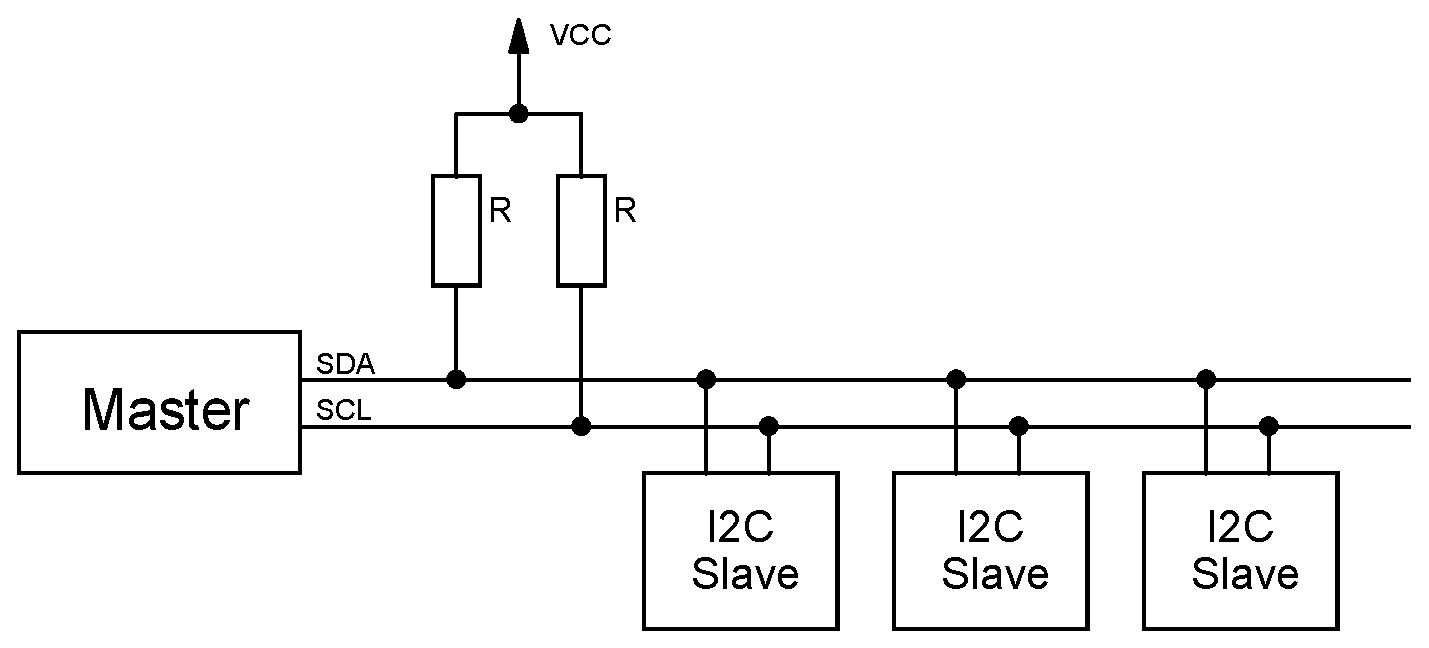
\includegraphics[width=0.9\linewidth]{i2c.eps}
	\caption{I$^{2}$C Master/Slaves}
	\label{figure:i2c}
\end{figure}

\pagebreak

\section{Implementation}
\subsection{Fluss- und Ablaufdiagramme}
\label{sec:flussablauf}
Um den Befehlsablauf speziell für die 1-Wire und I$^{2}$C-Schnittstelle im Code (siehe \ref{sec:codeimpref}) besser nachzuvollziehen, werden diese in Form von Fluss- bzw. Ablaufdiagrammen veranschaulicht.

\subsubsection{1-Wire-Temperaturmessung}
Der Ablauf der Temperaturmessung mit dem 1-Wire-Temperatursensor ist im nachfolgendem Flussdiagramm ersichtlich:

\begin{figure}[H]
	\centering
	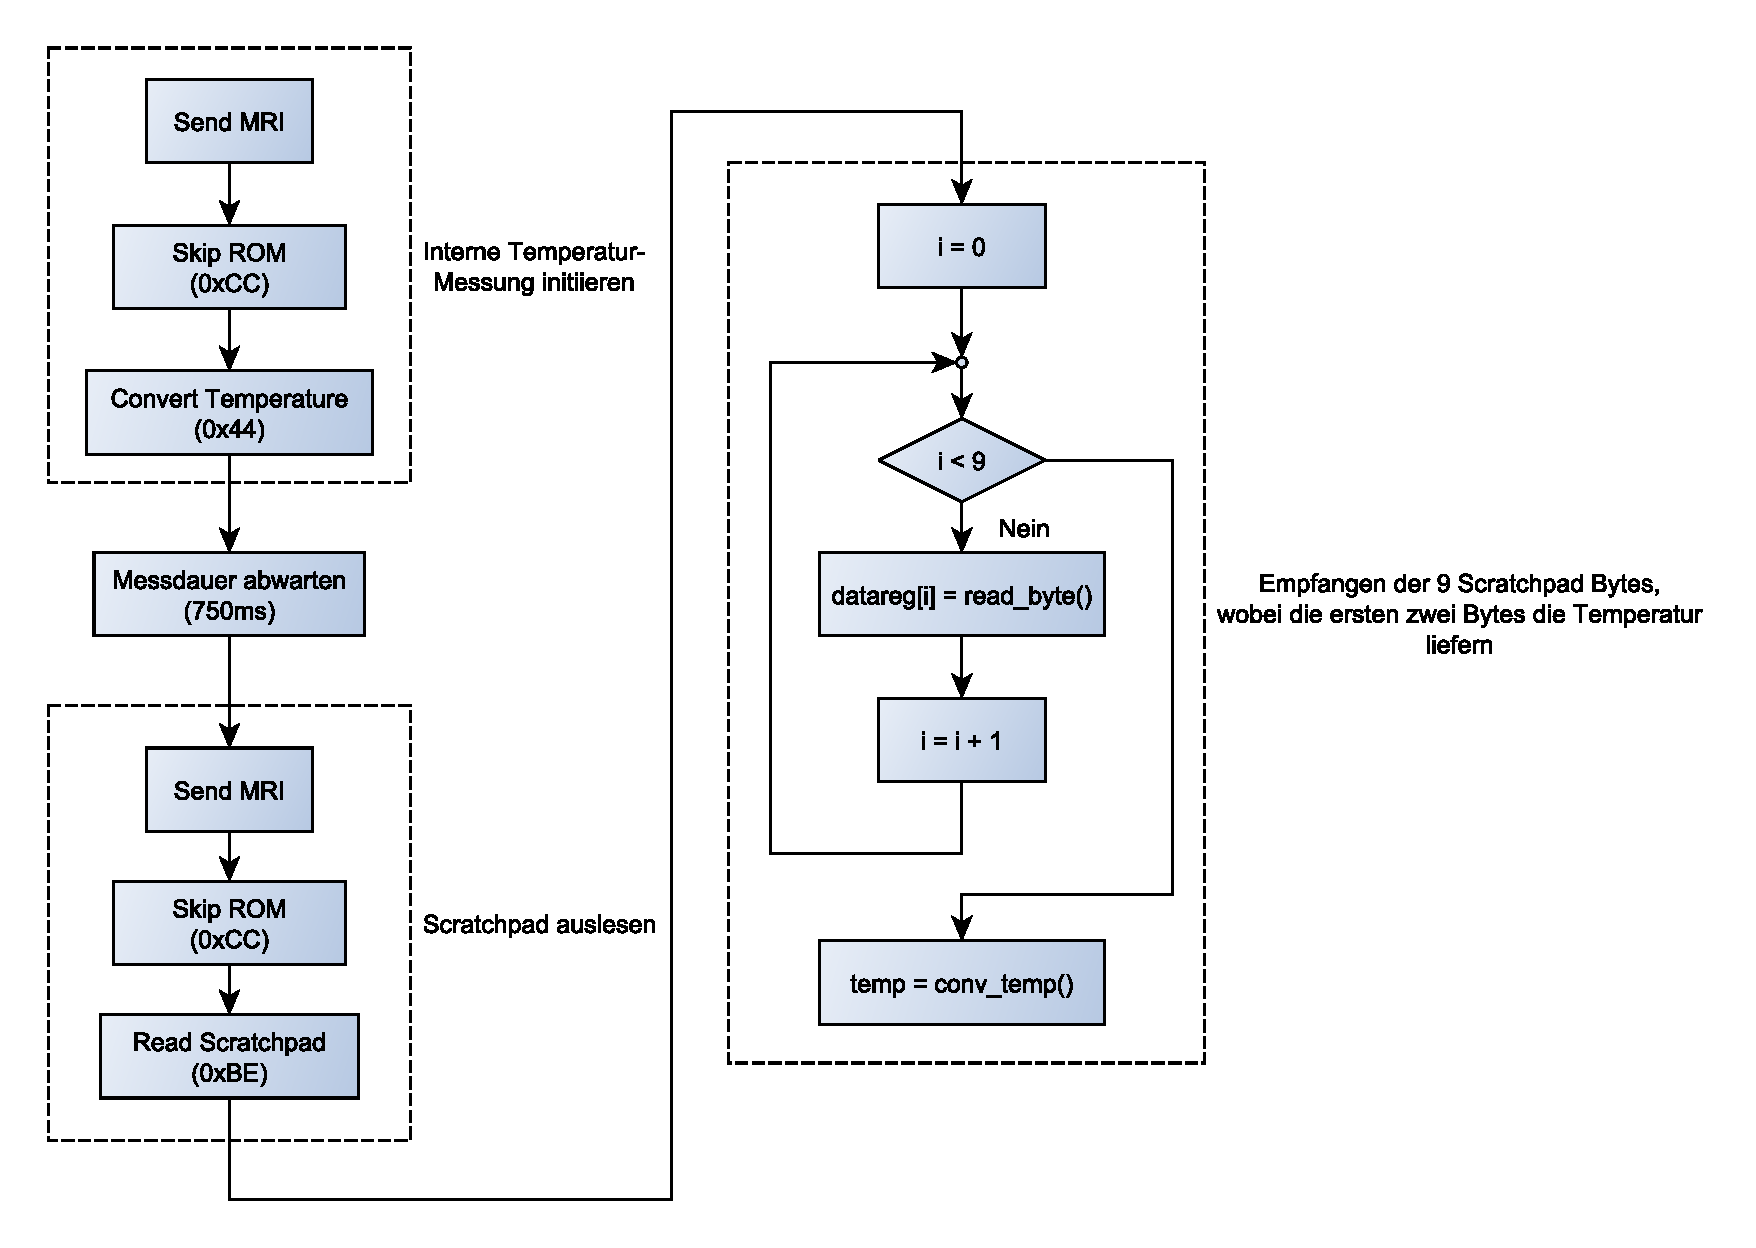
\includegraphics[width=1\linewidth]{temp_mess_flussdiagramm_V01}
	\caption{Flussdiagramm der Temperaturmessung}
	\label{figure:onewirefluss}
\end{figure}

\pagebreak

\subsubsection{I$^{2}$C/LCD-Display-Ansteuerung}
Nachfolgend wird die LCD-Display-Initialisierung über die I$^{2}$C-Schnittstelle dargestellt:

\begin{figure}[H]
	\centering
	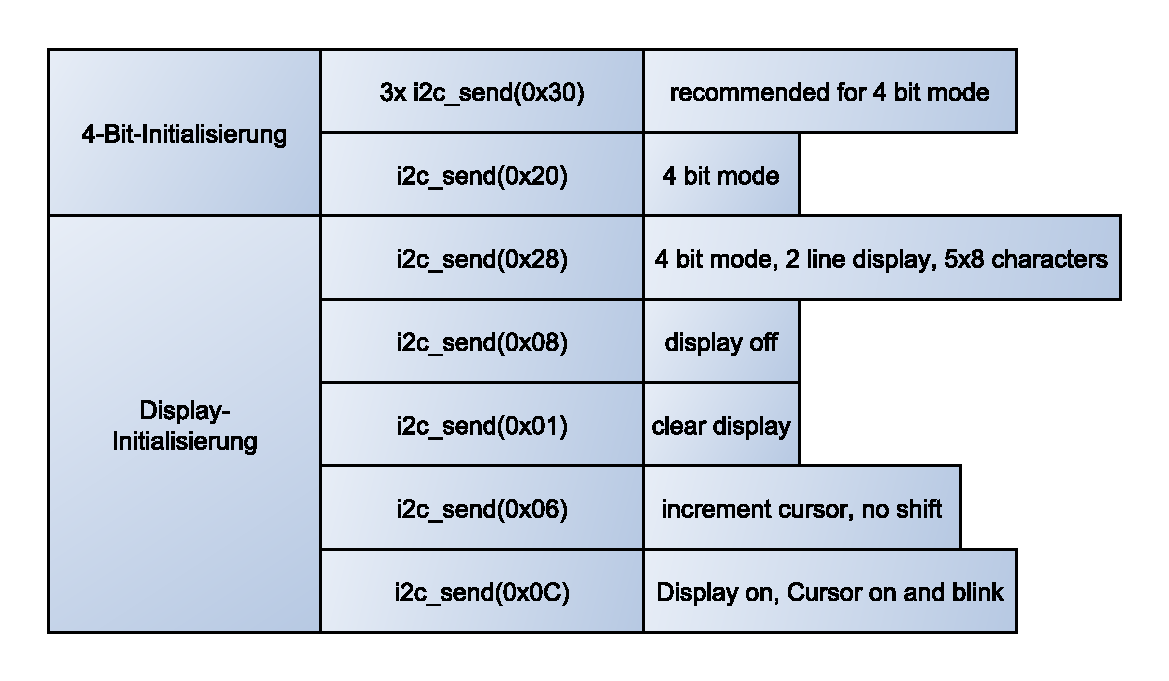
\includegraphics[width=0.9\linewidth]{i2c_lcd_init}
	\caption{Ablaufdiagramm der LCD-Display-Initialisierung}
	\label{figure:i2c_lcd_init}
\end{figure}

\pagebreak

\subsection{Code-Implementierung}
\label{sec:codeimpref}
Es folgen nun Code-Snippets der Temperaturmessung, der LCD-Display-Initialisierung und der Main-Funktion.
Dabei bauen die Code-Snippets auf den Diagrammen in \ref{sec:flussablauf} auf.
\subsubsection{1-Wire-Temperatursensor Code}
\begin{minipage}{\textwidth}
	\lstinputlisting[caption={Temperaturmessung}, label = {listing:sens}, firstline=117, lastline=140]{SENS_DS18X20.c}
\end{minipage}

\subsubsection{LCD-I$^{2}$C-Display-Initialisierungscode}
\begin{minipage}{\textwidth}
	\lstinputlisting[caption={LCD-Display-Initialisierung}, label = {listing:lcd_i2c_init}, firstline=66, lastline=95]{LCD_I2C.c}
\end{minipage}

\pagebreak

\subsubsection{Main-Funktion}
\begin{minipage}{\textwidth}
	\lstinputlisting[caption={Main-Funktion}, label = {listing:main}, firstline=59, lastline=124]{main.c}
\end{minipage}

\pagebreak

\section{Messungen}
\subsection{1-Wire-Temperatursensor}
\textbf{Messungen mit dem Logic-Analyzer:} \\
Messinitiierung:
\begin{figure}[H]
	\centering
	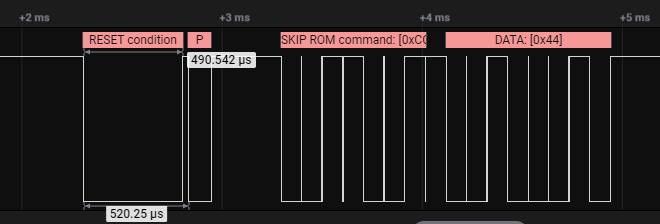
\includegraphics[width=0.9\linewidth]{Messinitialisierung_1wire_Logic}
	\caption{Messinitierung des Temperatursensors - Logic Analyzer}
	\label{figure:Messinitialisierung_1wire_Logic}
\end{figure}

Start der $750\mu s$ Messdauer:
\begin{figure}[H]
	\centering
	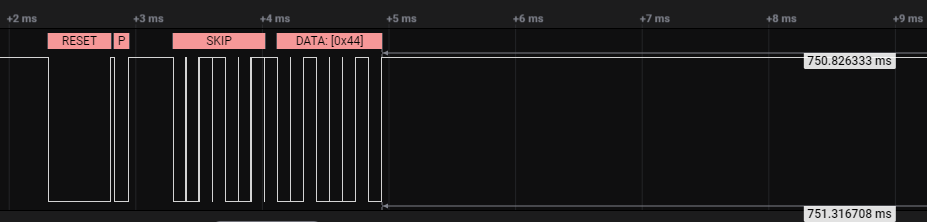
\includegraphics[width=1\linewidth]{Messdauer_750ms_1wire_Logic}
	\caption{Start der Messdauer - Logic Analyzer}
	\label{figure:Messdauer_750ms_1wire_Logic}
\end{figure}

Auslesen der Temperatur aus dem Scratchpad:
\begin{figure}[H]
	\centering
	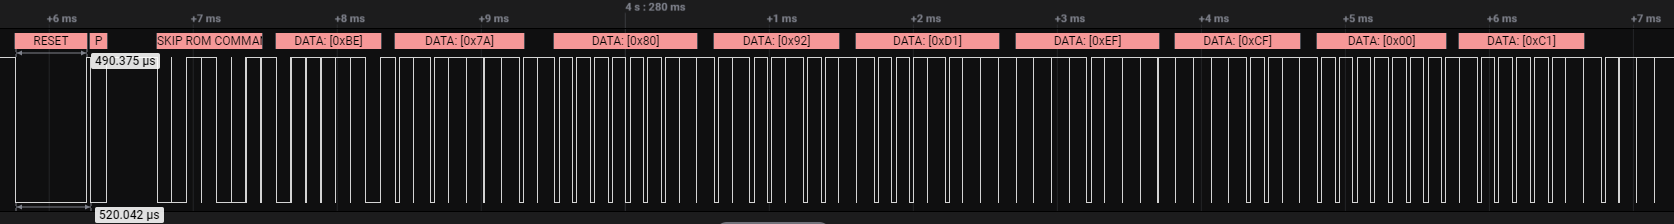
\includegraphics[width=1\linewidth]{scratchpad_1wire_Logic}
	\caption{Auslesen der Temperatur aus dem Scratchpad - Logic Analyzer}
	\label{figure:scratchpad_1wire_Logic}
\end{figure}

\pagebreak

\textbf{Messungen mit dem Oszilloskop:} \\
Messinitiierung:
\begin{figure}[H]
	\centering
	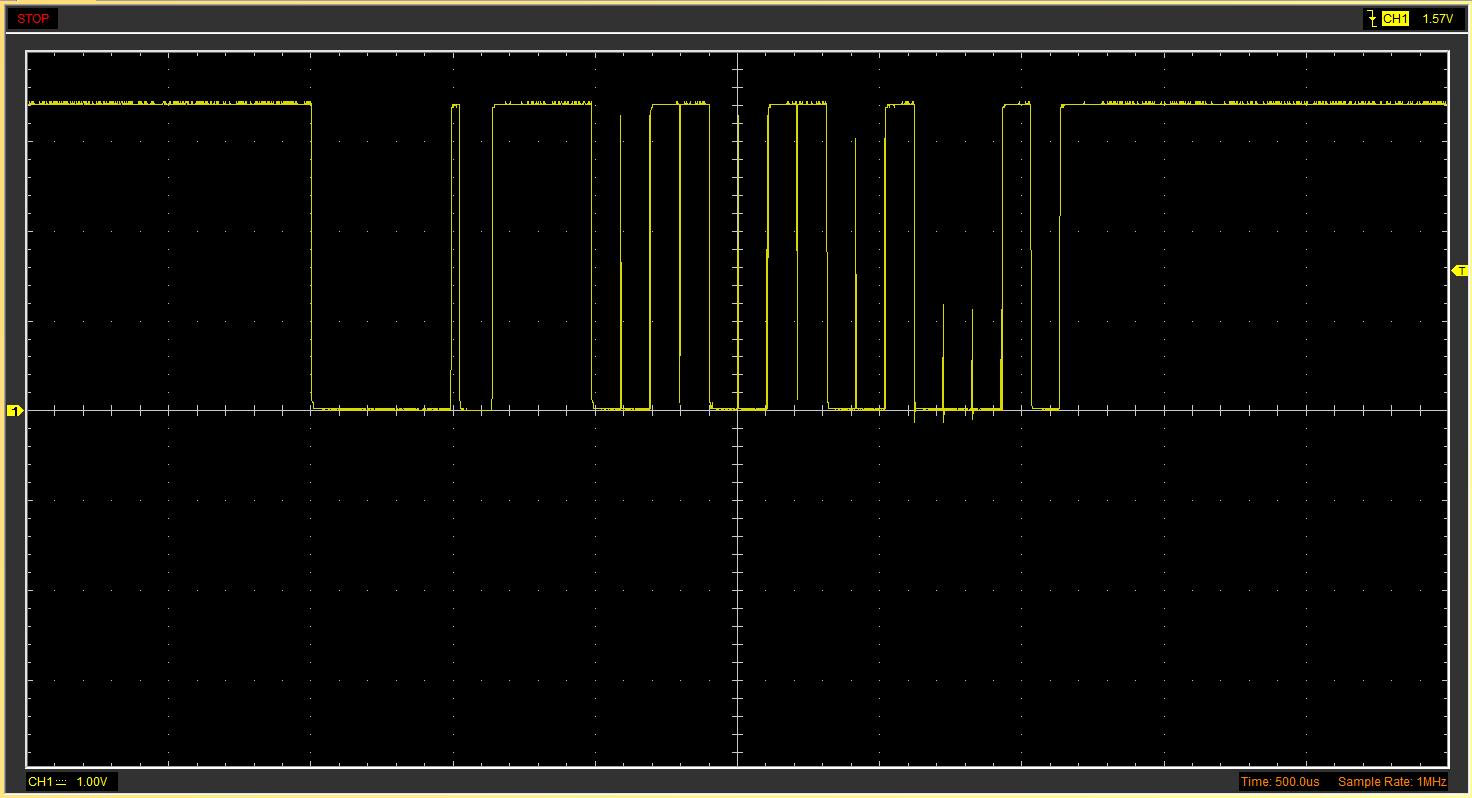
\includegraphics[width=0.9\linewidth]{Messinitialisierung_1wire_Oszi}
	\caption{Messinitierung des Temperatursensors - Oszilloskop}
	\label{figure:Messinitialisierung_1wire_Oszi}
\end{figure}

Auslesen der Temperatur aus dem Scratchpad:
\begin{figure}[H]
	\centering
	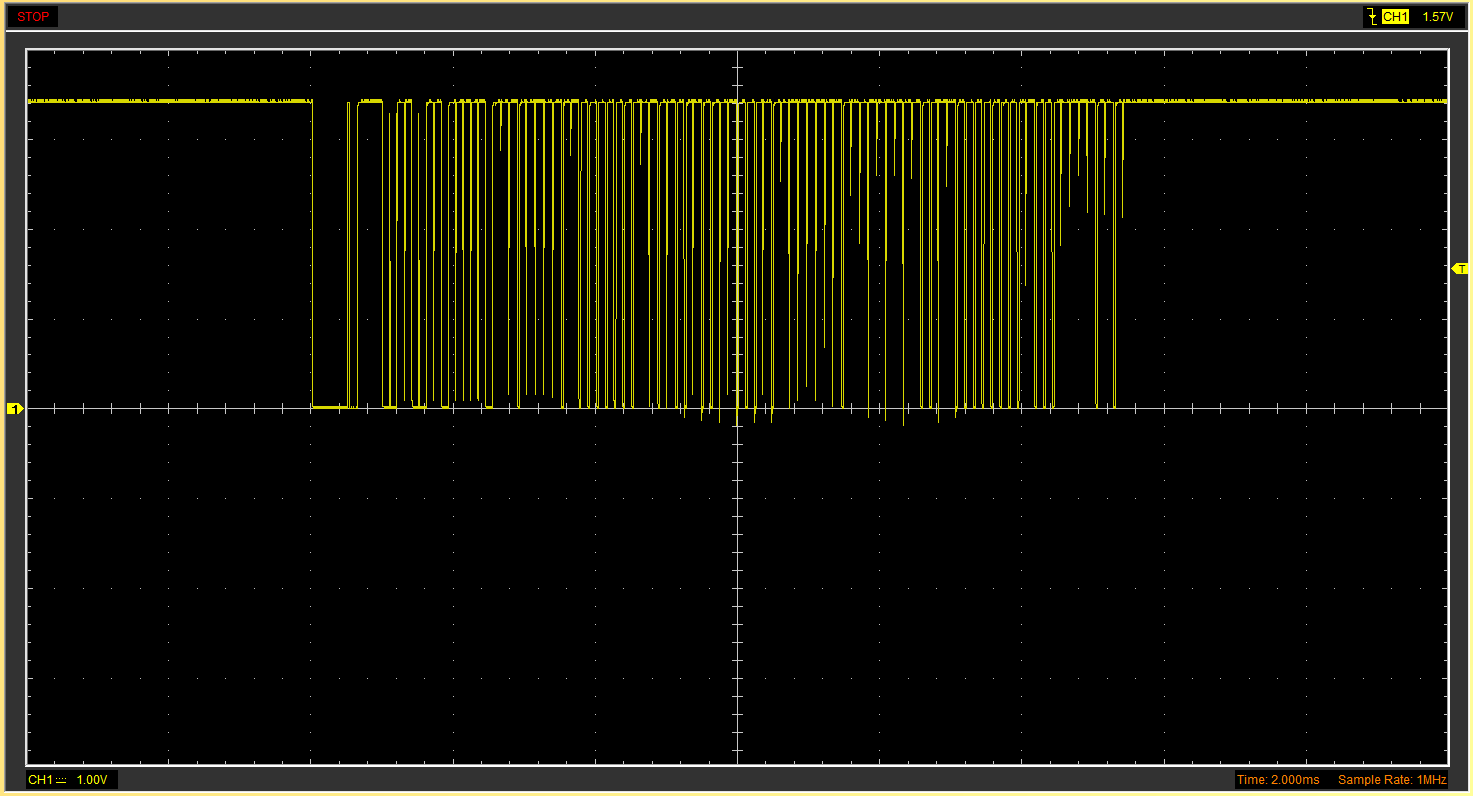
\includegraphics[width=1\linewidth]{scratchpad_1wire_Oszi}
	\caption{Auslesen der Temperatur aus dem Scratchpad - Oszilloskop}
	\label{figure:scratchpad_1wire_Oszi}
\end{figure}

\pagebreak

\subsection{I$^2$C/LCD Interfacing}
\uline{Bemerkung:} Die I$^2$C-Messung wird nur mit dem Logic Analyzer durchgeführt. \\\\
Komplette I$^2$C-Initialisierung:
\begin{figure}[H]
	\centering
	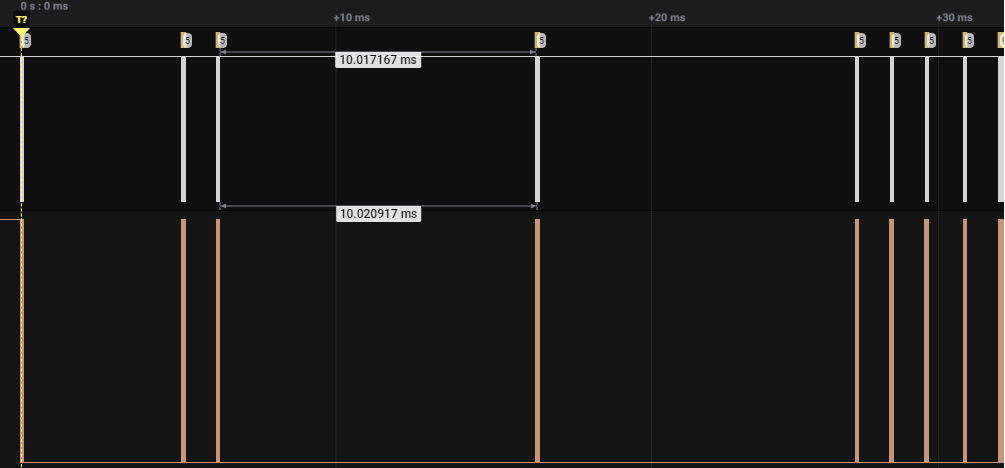
\includegraphics[width=1\linewidth]{lcd_i2c_init}
	\caption{I$^2$C-Initialisierung}
	\label{figure:lcd_i2c_init}
\end{figure}

Teilausschnitt der Initialisierung, Sende den Befehl 0x30 ans Display:
\begin{figure}[H]
	\centering
	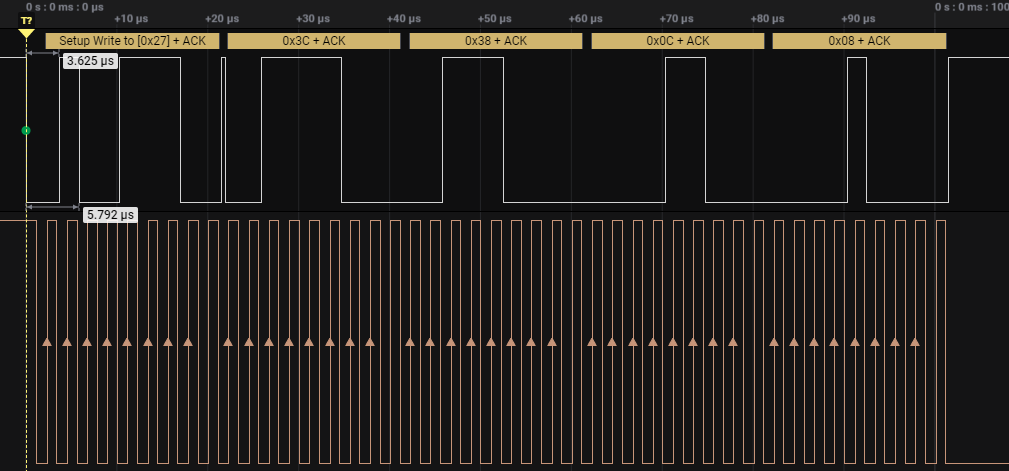
\includegraphics[width=1\linewidth]{lcd_i2c_send_cmd_0x30}
	\caption{Teil-Ausschnitt der I$^2$C-Initialisierung}
	\label{figure:lcd_i2c_send_cmd_0x30}
\end{figure}
\pagebreak

\section{Lessons Learned}
\begin{description}
	\item[Versorgungsproblem:]\hfill \\
	Nachdem die I$^2$C-Schnittstelle für das LCD-Display fertig programmiert wurde, gab es Probleme mit dem Kontrast bzw. mit der Helligkeit des Displays. Der ausgegebene Text war schlecht erkennbar. \\
	Die Lösung war es den Microcontroller nicht nur über die ST-Link-Schnittstelle anzuschließen, sondern zusätzlich über die USB Schnittstelle zu versorgen.
	Dadurch konnte die notwendige Stromzufuhr für das LCD-Display bereit gestellt werden.
	\item[Unnötige I$^2$C-Pull-Up-Widerstände:]\hfill \\
	Der erste Hardware-Aufbau der I$^2$C-Schnittstelle wurde mit zwei 10k$\ohm$ Widerständen durchgeführt. Eine nähere Begutachtung der Beschaltung des I2C/LCD-Interface Moduls im Datenblatt zeigte, dass dort entsprechende Pull-Up-Widerstände bereits vorhanden sind. Daher konnte auf die Widerstände verzichtet werden.
	\item[I$^2$C-Messung mit dem Logic-Analyzer:]\hfill \\
	Der Logic-Analyzer bietet die Möglichkeit mit einer Auto-Mess-Funktion die übertragenen Daten direkt zu intepretieren. Diese Funktion wird bei der I$^2$C-Messung verwendet, um
	die Übertragung der SDA- und SCL-Leitung genau nachzuvollziehen. Dabei gab es aber das Problem, dass die Auto-Messung die Daten nicht intepretieren konnte. \\
	Das Problem lag in der Zuweisung der Leitungen: Die SDA- und SCL-Leitung wurden hardwaremäßig vertauscht an den Logic-Analyzer angeschlossen, daher konnte die Messsoftware die Leitung auch nicht interpretieren. Als die Leitungen richtig angeschlossen wurden, konnte die Messung ohne Probleme durchgeführt werden.
	\item[Dauer der Temperaturmessung:]\hfill \\
	Der Temperatursensor liefert zeitweise erst nach ca. 10 Minuten bis 1h nach der ersten Messung einen korrekten Temperaturwert.
	Daraus kann geschlossen werden, dass der Sensor eher träge auf grobe Temperaturschwankungen reagiert.
\end{description}

\pagebreak
\listoffigures
\lstlistoflistings

\end{document}